\section{k3s}
K3s is described by the manufacturer as lightweight Kubernetes distribution designed for production workloads in unattended, resource-constrained, remote locations or inside IoT appliances \cite{k3s}. In short k3s is a Kubernetes distribution for IoT and edge computing. It is packed into a single binary with demand for minimal dependencies \cite{Thoughtworks2020}. K3s also supports the ARM processor architectures ARM64 and AMRv7 \cite{k3s}.

K3s requires the following dependencies for working correctly.

\begin{table}[H]
    \begin{tabularx}{\textwidth}{|X|X|} \hline
        \rowcolor{inovexBlue} 
        {\color[HTML]{FFFFFF} Dependency} & {\color[HTML]{FFFFFF} Description} \\ \hline
        containerd & Container runtime \\ \hline
        Flannel & Network fabrics designed to use Kubernetes API \cite{Flannelcontributors2021}. Functions as \acrfull{CNI} \\ \hline
        CoreDNS & Internal DNS service e.g. connecting to services by name \cite{TheCoreDNSAuthors2021} \\ \hline
        Host utilities & iptables, socat, etc \\ \hline
        Ingress controller & The ingress controller traefik is preinstalled \cite{TraefikLabs} \\ \hline
        Embedded service loadbalancer & Distributing work loads to different pods  \\ \hline
        Embedded network policy controller & Control traffic flow \\ \hline
    \end{tabularx}
    \caption{Packages/Dependencies included in k3s \cite{RancherDocs2020}.}
    \label{tab:pakc-dep-included-in-k3s}
\end{table}

In figure \ref{fig:how-it-works-k3s} the overall architecture of k3s is shown. The system contains a k3s server and a k3s agent consisting of various services and components.

\begin{figure}[H]
  \centering
  \includesvg[width=\textwidth]{assets/k3s/how-it-works-k3s.svg}
  \caption{k3s internal architecture of k3s server and k3s agent \cite{k3s}.}
  \label{fig:how-it-works-k3s}
\end{figure}

\paragraph{K3s server:} The k3s server serves the Kubernetes API and runs the Kubernetes control plane services. The control plane manages the worker nodes. The word worker nodes refer to machines with the k3s agent. The control plane consists of several services/components to make global decisions about the cluster like scheduling pods. These services/components also react to cluster events, for example adding pods when a deployment’s replica configuration was changed \cite{Rancher} \cite{kubernetes-components}.

\paragraph{K3s agent:} The k3s agent, or in the Kubernetes context also called worker node, is maintaining running pods and providing the Kubernetes runtime environment. Each agent must establish at least one connection to a corresponding k3s server instance. The k3s agents are getting their instructions from the k3s servers \cite{Rancher} \cite{kubernetes-components}.

%%%%%%%%%%%%%%%%%%%%%%%%%%%%%%%%%%%%%%%%%%%%%%%%%%%%%%%%%%%%%%%%%%%%%%%%%%%%%%%%%%%%%%%%%%%%
%%%%%%%%%%%%%%%%%%%%%%%%%%%%%%%%%%%%%%%%%%%%%%%%%%%%%%%%%%%%%%%%%%%%%%%%%%%%%%%%%%%%%%%%%%%%
\subsection{Use case implementation}
Figure \ref{fig:k3s-arch-overview} shows a simplified overview about the architecture. Everything inside the light blue rectangle is part of the k3s cluster. The yellowed rectangles, inside the blue ones, represent the Kubernetes namespaces and their content. The use case architecture consists of several Kubernetes namespaces to distinguish the services from the other services. For example, the \textit{mqtt} namespace contains a MQTT broker cluster while the \textit{default} namespace contains all services which process the messages from the MQTT brokers.

\newpage
\begin{figure}[H]
    \centering
    \fontsize{8}{10}\selectfont
    \def\svgwidth{\textwidth}
    \input{assets/k3s/arch-overview.drawio.pdf_tex}
    \caption{Simplified overview about the architecture.}
    \label{fig:k3s-arch-overview}
\end{figure}
\newpage


\subsubsection*{Node setup}
All three nodes and the fourth node, which was added later, were provisioned with the configuration management Ansible\footnote{\url{https://www.ansible.com/}} tool. With this tool, a given configuration was installed on each of the nodes. The configuration includes the installation and cluster creation of k3s and necessary prerequisite steps like enabling cgroup or enabling IPv4 and IPv6 forwarding. All Ansible configuration files are included inside the Git repository\footnote{\url{https://github.com/lukaskirner/edge-platforms-evaluation}} which allow an automatic cluster setup.

\subsubsection*{Client devices}\label{subsubsec:k3s-client-devices}
All three devices BMP280, MQ2 and Ventilator use the PubSubClient from Nick O'Leary to subscribe and publish to the MQTT broker. To make the program simple for each sensor/actor, a little shared library was written to connect with the PubSubClient to the local MQTT broker by providing a simple configuration. The library handles the entire connection process form establishing a connection to the next WiFi access point over to connecting to the local MQTT broker. Listing \ref{lst:k3s-client-devices-config} shows the configuration object of shared library.

\begin{lstlisting}[caption={ThesisEdge library configuration object.},label={lst:k3s-client-devices-config},captionpos=b]
ThesisEdge edge_config = {
  .wifi_ssid = <wifi_ssid>,
  .wifi_pass = <wifi_password>,
  .mqtt_clientId_prefix = <client_id>,
  .mqtt_broker = <mqtt_broker_host>,
  .mqtt_port = <mqtt_port>,
};
\end{lstlisting}


\subsubsection*{MQTT}\label{subsubsec:k3s-mqtt}
This edge computing platform does not come with any built in MQTT broker like others do, therefore an own MQTT cluster needs to be deployed. The EMQX\footnote{\url{https://www.emqx.io/}} \gls{MQTT} broker allows a deployment in cluster mode, which allows this setup to deploy at least one or more brokers to each of to k3s nodes. EMQX was chosen due to its ability to scale well horizontally and its better performance in message throughput compared to its competitors \cite{Koziolek2020}. For simplicity the EMQX brokers can be installed by using an official Helm chart\footnote{A Helm chart is a collection of files that describe a related set of Kubernetes resources \cite{HelmAuthorsCharts}} \footnote{\url{https://github.com/emqx/emqx-rel/tree/master/deploy/charts/emqx}} from the vendor EMQ Technologies. The Helm chart includes nearly everything from automatically deploy the brokers in cluster mode to exposing a web dashboard with the ingress controller. In addition to the default configuration, the \textit{emqx\_prometheus} plugin can be installed to export metrics about the \gls{MQTT} brokers. These metrics will then be pushed to a Prometheus push gateway and can then be further used for monitoring. The Prometheus can be installed and configured like shown in listing \ref{lst:k3s-emqx-helm-values-prometheus}. To reach the brokers from outside the cluster an ingress in conjunction with a load balancer service is defined. This makes the MQTT cluster accessible for devices outside the platform and also evenly distributes the workload of incoming connections to the cluster.

\begin{lstlisting}[caption={Build emergency container image for ARM with Jib.},label={lst:k3s-emqx-helm-values-prometheus},captionpos=b]
emqxConfig:
    EMQX_LOADED_PLUGINS: "<...>,emqx_prometheus"
    EMQX_PROMETHEUS__PUSH__GATEWAY__SERVER: <internal_url_to_pushgateway>
    EMQX_PROMETHEUS__INTERVAL: 15000
    ...
\end{lstlisting}

%%%%%%%%%%%%%%%%%%%%%%%%%%%%%%%%%%%%%%%%%%%%%%%%%%%%%%%%%%%%%%%%%%%%%%%%%%%%%%%%%%%%%%%%%%%%
\newpage
\subsubsection*{Detector service}\label{subsubsec:k3s-detector}
This detector service runs a small python program which triggers machine learning inference on every received image. The image is received over a specific MQTT topic, \textit{sensor/camera}. The received image is Base64 encoded and must be decoded for further processing. Like all services this service needs to be build for the ARM processor architecture to run on the example cluster.

\bigskip
To access hardware, in this case USB, on the host system the pod requires privileged access to do so. This can be enabled by a simple boolean attribute like shown in listing \ref{lst:k3s-detector-attach-tpu} at line seven. Not just the access to the USB port is necessary, additionally the pod must also be started on the correct node, where the TPU is attached to, otherwise there is no USB device to mount. Listing \ref{lst:k3s-detector-attach-tpu} shows the necessary additions to the pod configuration to mount the USB device and selecting the correct node. Note, the labeling of the nodes must be done manually before deploying the pod.

\begin{lstlisting}[caption={Give detector pod access to via USB attached TPU.},label={lst:k3s-detector-attach-tpu},captionpos=b]
...
spec:
  containers:
    - name: detector
      image: <container_image>
      securityContext:
        privileged: true
      volumeMounts:
        - mountPath: /dev/bus/usb
          name: usb
  nodeSelector:
    type: tpu # <-- pod with TPU attached is labeled 
  volumes:
    - name: usb
      hostPath:
        path: /dev/bus/usb
...
\end{lstlisting}
%%%%%%%%%%%%%%%%%%%%%%%%%%%%%%%%%%%%%%%%%%%%%%%%%%%%%%%%%%%%%%%%%%%%%%%%%%%%%%%%%%%%%%%%%%%%
\subsubsection*{Emergency Service}
The functionality of this service is explained in the subsection \ref{subsec:emergency-service}. The emergency service was built with Spring Boot 2.4.5 in conjunction with the \gls{JVM} programming language Kotlin. By using Eclipse's Paho\footnote{\url{https://www.eclipse.org/paho/}} \gls{MQTT} client the service subscribes to the MQTT topic \textit{sensor/\#} and publishes to the topic \textit{actor/ventilation} on certain temperature and gas value thresholds.

\bigskip
This service also needs to be compiled for the ARM architecture as the subsection \ref{subsec:compute-units} already noted, therefore the Google container tool Jib\footnote{\url{https://github.com/GoogleContainerTools/jib}} is used. Jib also allows the container building without an active docker daemon. To cross compile with Jib the base image inside the \textit{build.gradle.kts} file must be changed to an ARM processor image like shown in listing \ref{lst:k3s-emergency-service-build-gradle}.

\bigskip
The service can then be deployed to the k3s cluster using Kubernetes YAML configuration files. This service only requires a deployment specification, other specifications like a Kubernetes service or load balancer isn't necessary. The deployment file also hands in the Redis password by using environment variables.

\begin{lstlisting}[caption={Build emergency container image for ARM with Jib.},label={lst:k3s-emergency-service-build-gradle},captionpos=b]
jib {
    from {
        image = "docker.io/arm64v8/openjdk:11-slim"
    }
    ...
}
\end{lstlisting}

\paragraph{Redis Cluster:}
The emergency service uses a Redis cluster to store the current state of ventilation start/stop events. For redundancy purpose, a cluster is set up. The Redis cluster can be set up with the Bitnami Helm chart\footnote{\url{https://github.com/bitnami/charts/tree/master/bitnami/redis}} which allows convenient configuration via variables.
    
%%%%%%%%%%%%%%%%%%%%%%%%%%%%%%%%%%%%%%%%%%%%%%%%%%%%%%%%%%%%%%%%%%%%%%%%%%%%%%%%%%%%%%%%%%%%
\subsubsection*{Database service}\label{subsubsec:k3s-database-service}
This service is represented as a time series database. The time series storage consist of two services. First the Time series database InfluxDB\footnote{\url{https://www.influxdata.com/}}, which stores the MQTT messages and second the Telegraf agent. The database itself is not capable of subscribing to the MQTT topics itself. Therefore, the program \textit{Telegraf}\footnote{\url{https://www.influxdata.com/time-series-platform/telegraf/}} from InfluxData will handle the subscribing to the specified MQTT topics. To store the incoming MQTT messages Telegraf transforms them to the InfluxDB format. For simplification purposes both, InfluxDB and Telegraf, can be installed with HELM and corresponding configuration files. Listing \ref{lst:k3s-timeseries-telegraf-config} shows one configuration of Telegraf which must be made for subscribing to MQTT topics and storing the received messages to the InfluxDB. The configuration is very simple and split into \textit{inputs} where attributes define the connection to the MQTT broker and \textit{outputs} which define the connection parameters to the InfluxDB.

\begin{lstlisting}[caption={HELM configuration for storing MQTT messages into InfluxDB by using Telegraf.},label={lst:k3s-timeseries-telegraf-config},captionpos=b]
config:
  inputs:
    - mqtt_consumer:
        servers: ["tcp://<name>.<namespace>.svc.cluster.local:1883"]
        topics: ["sensor/#", "actors/#", ...]
        client_id: "telegraf-sensors-actors"
        data_format: "json"
        json_strict: true
    ...
outputs:
    - influxdb:
        urls:
          - "http://<internal_influxdb_url>:8086"
        database: <database_name>
\end{lstlisting}

%%%%%%%%%%%%%%%%%%%%%%%%%%%%%%%%%%%%%%%%%%%%%%%%%%%%%%%%%%%%%%%%%%%%%%%%%%%%%%%%%%%%%%%%%%%%
\subsubsection*{Monitoring service}
A collection of services which represent the monitoring from subsection \ref{subsec:monitoring-service}. This collection includes the Kubernetes state metrics collector, the Prometheus\footnote{\url{https://prometheus.io/}} monitoring solution and Grafana\footnote{\url{https://grafana.com/}} as visualization dashboard. Like many other services, these three services can be installed with HELM charts too. The default configuration of all three HELM charts work for this example out of the box. Optionally, Grafana can be preconfigured to skip data source configuration via the interface. By creating or importing existing dashboards into Grafana, images like figure \ref{fig:k3s-grafana-k3s-metrics} can be produced.

\begin{figure}[H]
    \centering
    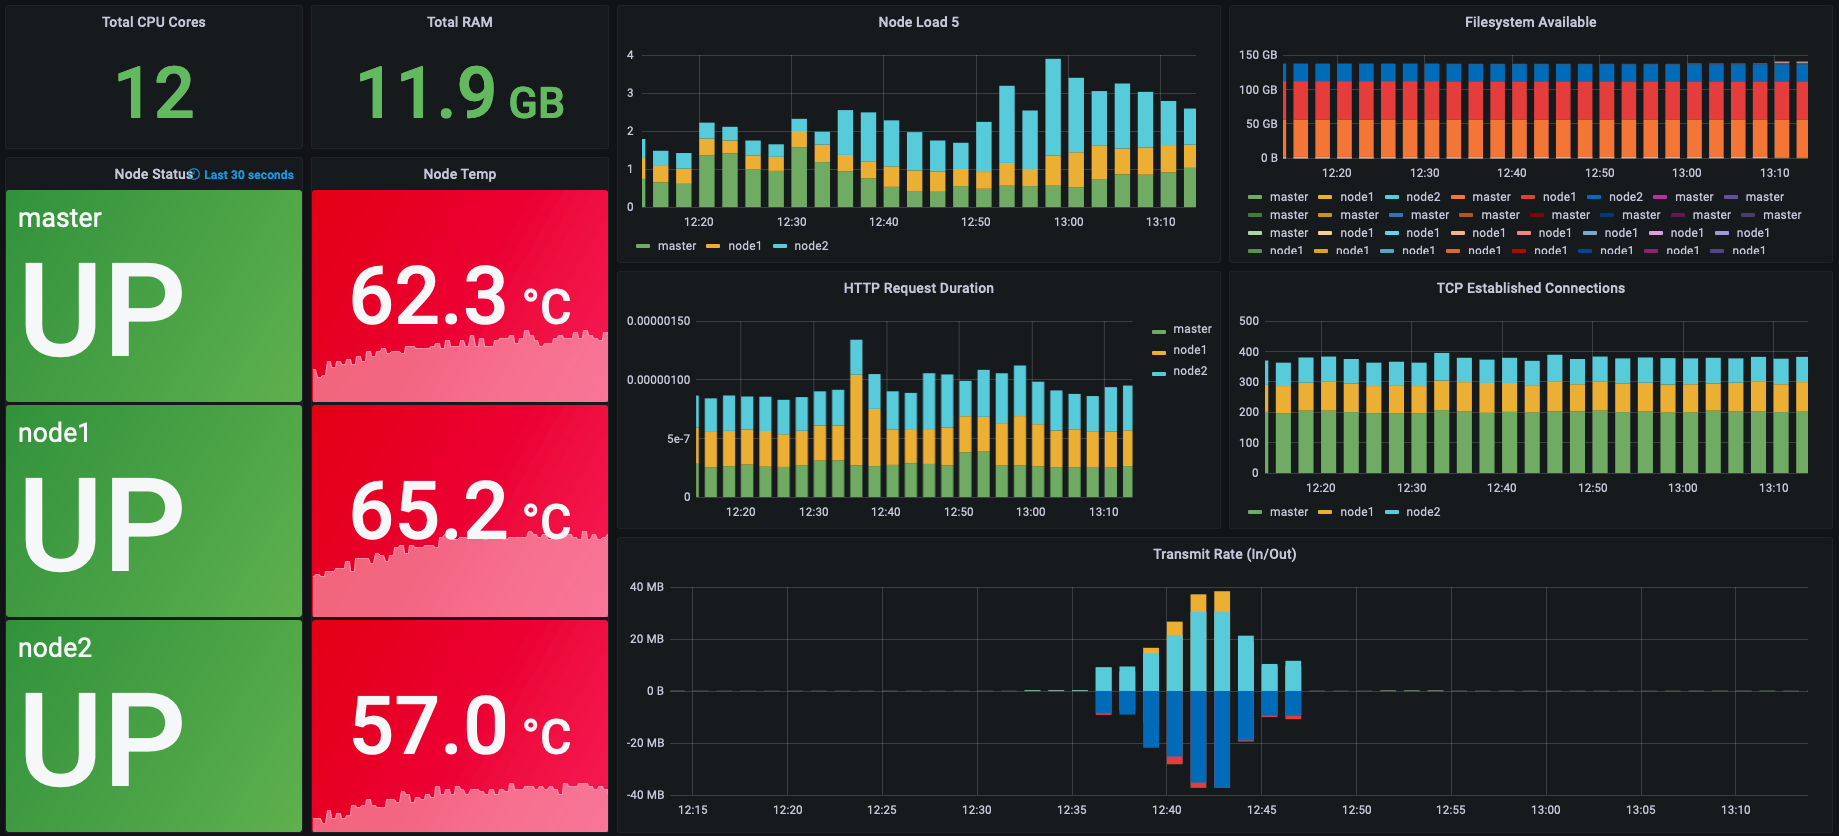
\includegraphics[width=\textwidth]{assets/k3s/screenshots/grafana-k3s-metrics.png}
    \caption{K3s metrics on Grafana dashboard.}\label{fig:k3s-grafana-k3s-metrics}
\end{figure}

Besides using Prometheus as data source, the internal InfluxDB from subsection \ref{subsubsec:k3s-database-service} can also be used to provide data for visualization in Grafana. Figure \ref{fig:k3s-grafana-sensor-temperature-png} shows the average temperature of all BMP280 sensors by requesting the values form the InfluxDB.

\begin{figure}[H]
    \centering
    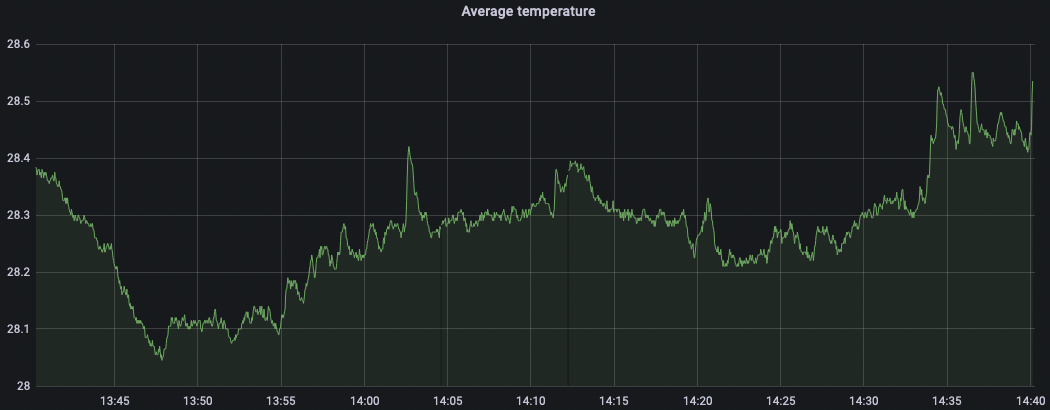
\includegraphics[width=\textwidth]{assets/k3s/screenshots/grafana-sensor-temperature-png.png}
    \caption{Average temperature of BMP280 sensors. Values provided by internal InfluxDB.}\label{fig:k3s-grafana-sensor-temperature-png}
\end{figure}

%%%%%%%%%%%%%%%%%%%%%%%%%%%%%%%%%%%%%%%%%%%%%%%%%%%%%%%%%%%%%%%%%%%%%%%%%%%%%%%%%%%%%%%%%%%%
